%Master File:lectures.tex

\lesson{Stochastic Gradient Descent}
\vspace{-1cm}
\begin{center}
  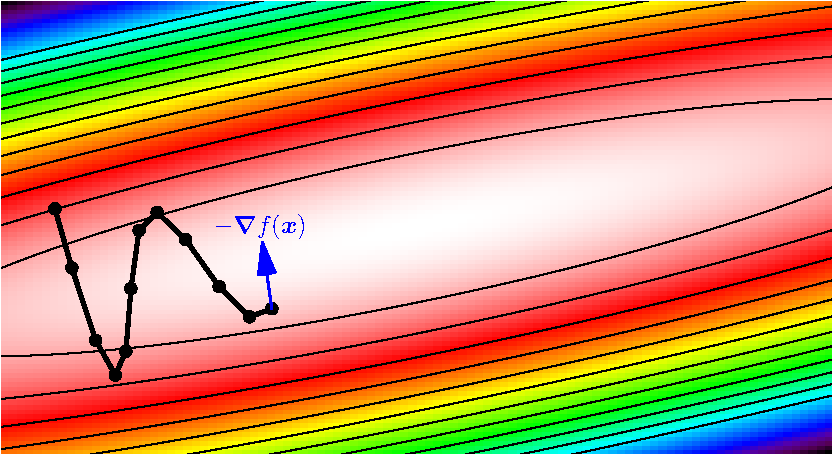
\includegraphics[width=0.9\linewidth]{momentumDynamics-23}
\end{center}
\keywords{SGD, momentum, step size, ADAM}
%%%%%%%%%%%%%%%%%%%%%%% Next Slide %%%%%%%%%%%%%%%%%%%%%%%
\renewcommand{\Outline}{%
\begin{slide}
\section[1]{Outline}

\begin{minipage}{12cm}\raggedright
  \begin{enumerate}\squeeze
    \outlineitem{SGD}{sgd}
    \outlineitem{Momentum}{momentum}
    \outlineitem{Loss Landscapes}{landscapes}
  \end{enumerate}
\end{minipage}\hfill
\begin{minipage}{10cm}
  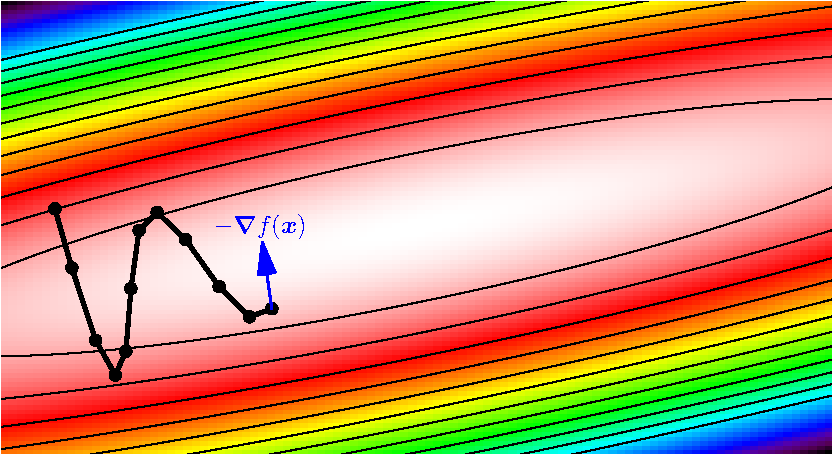
\includegraphics[width=10cm]{momentumDynamics-23}
\end{minipage}
\end{slide}
\addtocounter{outlineitem}{1}
}

\setcounter{outlineitem}{1}

%%%%%%%%%%%%%%%%%%%%%%% Next Slide %%%%%%%%%%%%%%%%%%%%%%%
\Outline % Motivation
\toptarget{firstoutline}
%%%%%%%%%%%%%%%%%%%%%%% Next Slide %%%%%%%%%%%%%%%%%%%%%%%

\begin{slide}
\section{The Next Step}

\begin{PauseHighLight}
  \begin{itemize}
  \item In most machine learning problems we design a network and a
    loss function\pause
  \item The rest requires simple optimisation\pause
  \item Although Newton and Quasi-Newton methods ensure rapid
    convergence for many tasks this apparent advantage is
    delusionary\pause
  \item Since the raise of deep learning, gradient descent and its
    variants have become dominant\pause    
  \end{itemize}
\end{PauseHighLight}

\end{slide}

%%%%%%%%%%%%%%%%%%%%%%% Next Slide %%%%%%%%%%%%%%%%%%%%%%%

\begin{slide}
\section{Mini-Batch Learning}

\begin{PauseHighLight}
  \begin{itemize}
  \item Rather than computing the gradient of the loss function, e.g.
    \begin{align*}
      \grad L_{\mathcal{D}}(\bm{w}) = \grad \sum_{(\bm{x},y)\in\mathcal{D}}
      L\!\left( \strut f(\bm{x}|\bm{w}), y \right)^2\pause
    \end{align*}
  \item We often compute an approximation
    \begin{align*}
      \grad L_{\mathcal{B}}(\bm{w})
      = \grad \sum_{(\bm{x},y)\in\mathcal{B}}
      L\!\left( \strut f(\bm{x}|\bm{w}), y \right)^2
    \end{align*}
  \item where $\mathcal{B}\subset\mathcal{D}$ is a randomly sampled
    subset of the training set\pause
  \item Usually $|\mathcal{B}| \ll |\mathcal{D}|$\pause
  \end{itemize}
\end{PauseHighLight}

\end{slide}

%%%%%%%%%%%%%%%%%%%%%%% Next Slide %%%%%%%%%%%%%%%%%%%%%%%

\begin{slide}
  \section{Stochastic Gradient Descent}

\begin{PauseHighLight}
  \begin{itemize}
  \item Stochastic gradient descent (SGD) follows the gradient of
    mini-batches\pause
  \item Computationally this is efficient because it is much quicker to
    compute $\grad L_{\mathcal{B}}(\bm{w})$ than $\grad
    L_{\mathcal{D}}(\bm{w})$\pause
  \item The batch gradients add noise (are stochastic) as we are only
    sampling the dataset\pause
  \item This noise might help escape local-minima\pause{} (but I'm not sure
    there is compelling evidence for this)\pauseb
  \item Taking many smaller steps of approximate gradients reduces the
    likelihood of divergence\pause
  \end{itemize}
\end{PauseHighLight}


\end{slide}

%%%%%%%%%%%%%%%%%%%%%%% Next Slide %%%%%%%%%%%%%%%%%%%%%%%

\begin{slide}
  \section{Automatic Differentiation}

\begin{PauseHighLight}
  \begin{itemize}
  \item For gradient descent we need to compute the gradient\pause
  \item For most of my life this was just a pain\pause
  \item You guys have it easy, modern deep learning frameworks do this
    for you automatically\pause
  \item This is a \textit{game changer}!\pause{}  We are no longer afraid of
    large models\pause
  \item We can differentiate through algorithms allowing us to
    training incredible sophisticated networks\pause
  \end{itemize}
\end{PauseHighLight}


\end{slide}

%%%%%%%%%%%%%%%%%%%%%%% Next Slide %%%%%%%%%%%%%%%%%%%%%%%

\begin{slide}
\section{Convergence}

\begin{PauseHighLight}
  \begin{itemize}
  \item Asymptotic convergence of gradient descent (and SGD) is slower
    than quasi-Newton methods\pause
  \item But there are three reasons why we don't really care\pause
    \begin{itemize}
    \item For complex models we spend a lot of time before we are
      close to a quadratic minima where asymptotic convergence kicks
      in\pause
    \item These days we often use ReLUs (rectified linear units) which
      are non-analytic.  The convergence we discussed depends on a
      Taylor expansion that assumes analyticity\pause
    \item We want to minimise the generalisation error, but are only
      minimising a poor surrogate, namely the training error\pause
    \end{itemize}
        
  \end{itemize}
\end{PauseHighLight}

\end{slide}



%%%%%%%%%%%%%%%%%%%%%%% Next Slide %%%%%%%%%%%%%%%%%%%%%%%
\Outline %  Momentum
%%%%%%%%%%%%%%%%%%%%%%% Next Slide %%%%%%%%%%%%%%%%%%%%%%%

\begin{slide}
\section[-2]{Step Size}

\begin{rightImage}{eigspec}
\begin{PauseHighLight}
  \begin{itemize}
  \item The optimal step size depends on the gradient and the
    curvature (second derivative)\pause
  \item For a quadratic minima the minimum is given by
    \begin{align*}
      x^* &= x - \frac{f'(x)}{f''(x)},
      &
      \bm{x}^* &= \bm{x} - \mat{H}^{-1} \grad f(\bm{x})\pause
    \end{align*}
  \item In high dimensions the Hessian $\mat{H}$ will have a spectrum
    of eigenvalues\pause
  \item This means there are different scales\pause
  \end{itemize}
\end{PauseHighLight}
  
\end{rightImage}

\end{slide}

%%%%%%%%%%%%%%%%%%%%%%% Next Slide %%%%%%%%%%%%%%%%%%%%%%%

\begin{slide}
\section{Gradient Descent}

\pauselevel{1:}
\pb\pause\pauselevel{=1}
\begin{center}
  \multipdf[width=\linewidth]{gradDescent}\pause
\end{center}
\end{slide}

%%%%%%%%%%%%%%%%%%%%%%% Next Slide %%%%%%%%%%%%%%%%%%%%%%%

\begin{slide}
\section{Avoiding Divergence}

\begin{PauseHighLight}
  \begin{itemize}
  \item We saw in the last lecture that gradient descent can actually
    diverge from a local optimum if you have a too big step size\pause
  \item If we use too large a step size we quickly get NaN
    errors\pause
  \item If we only use SGD the step size is determined by the largest
    eigenvalue of the Hessian\pause
  \item This seems impossibly slow\pauseb, but weirdly straightforward
    SGD is often used in deep learning\pauseb{} (although nearly always with momentum)\pauseb
  \end{itemize}
\end{PauseHighLight}

\end{slide}

%%%%%%%%%%%%%%%%%%%%%%% Next Slide %%%%%%%%%%%%%%%%%%%%%%%

\begin{slide}
  \section{Momentum}

  \begin{PauseHighLight}
    \begin{itemize}
    \item In high dimensions we zig-zag:
      \begin{itemize}
      \item stepping consistently in directions with low curvature
      \item jumping backwards and forwards past the minimum in
        directions with high curvature\pause
      \end{itemize}
    \item By introducing ``momentum'' we can increase our steps in
      low curvature directions and decrease it in high curvature
      directions
      \begin{align*}
        \bm{v}(t+1) &= \gamma \, \bm{v}(t) -  \eta\, \grad f(\bm{x}(t))\\
        \bm{x}(t+1) &= \bm{x}(t) + \bm{v}(t+1)\pause
      \end{align*}
      $0<\gamma<1$ is a damping term\pauseb 
    \end{itemize}
  \end{PauseHighLight}


\end{slide}


%%%%%%%%%%%%%%%%%%%%%%% Next Slide %%%%%%%%%%%%%%%%%%%%%%%

\begin{slide}
\section{Gradient Descent with Momentum}

\pauselevel{=1:}
\pb\pause\pauselevel{=1}
\begin{center}
  \multipdf[width=\linewidth]{momentumDynamics}\pause
\end{center}
\end{slide}

%%%%%%%%%%%%%%%%%%%%%%% Next Slide %%%%%%%%%%%%%%%%%%%%%%%

\begin{slide}
  \section{Adaptive Methods}

  \begin{PauseHighLight}
    \begin{itemize}
    \item A major difficulty of high dimensional optimisation is the
      existence of different scales\pause
    \item That is, there are some directions were we have to move a
      lot (low curvature), while other directions we have to make small
      steps\pause
    \item In adaptive methods we use a dynamic algorithm to rescale
      the step size of each parameter (weight)\pause
    \item We can think of this as a ``regularisation'' that makes our
      basins of attraction more spherical\pause
    \end{itemize}
  \end{PauseHighLight}

\end{slide}

%%%%%%%%%%%%%%%%%%%%%%% Next Slide %%%%%%%%%%%%%%%%%%%%%%%

\begin{slide}
\section[-2]{Rescaling Co-ordinates}

\pb\pauselevel{=1: 4}\pause\pauselevel{=1}
\begin{center}
  \multipdf[width=0.6\linewidth]{rescaleWeights}\pause
\end{center}
\end{slide}

%%%%%%%%%%%%%%%%%%%%%%% Next Slide %%%%%%%%%%%%%%%%%%%%%%%

\begin{slide}
  \section[-2]{AdaDelta}

  \begin{PauseHighLight}
    \begin{itemize}
    \item We want to rescale the coordinates in proportion to the
      curvature in that direction\pause
    \item To estimate the curvature we compute a running average of
      the squared gradients
      \begin{align*}
        S^g_i(t+1) = (1-\gamma)\, S^g_i(t) + \gamma \left(
        \pd{L_{\mathcal{B}}(\bm{w}(t))}{w_i(t)} \right)^2\pause
      \end{align*}
    \item To estimate the relative scale of the weights we compute a
      running average of the squared weights
      \begin{align*}
        S^w_i(t+1) = (1-\gamma) \, S^w_i(t) + \gamma \, w_i(t)^2\pause
      \end{align*}
     \end{itemize}
  \end{PauseHighLight}

\end{slide}

%%%%%%%%%%%%%%%%%%%%%%% Next Slide %%%%%%%%%%%%%%%%%%%%%%%

\begin{slide}
\section{AdaDelta}

\begin{PauseHighLight}
  \begin{itemize}
  \item The AdaDelta algorithm uses the update
    \begin{align*}
       w_i(t+1)
        = w_i(t) - \eta \,
        \sqrt{\frac{S^w_i(t+1)+\epsilon}{S^g_i(t+1)+\epsilon}}\,
        \pd{L_{\mathcal{B}}(\bm{w}(t))}{w_i(t)}\pause
    \end{align*}
  \item Note that we can rescale the weights or rescale the
    gradients yet the update would be the same\pause---this is one
    aspect of a covariant algorithm\pauseb
  \item Because we are adaptively changing our step size we can use a
    single step size throughout the optimisation\pause
  \end{itemize}
\end{PauseHighLight}

\end{slide}

%%%%%%%%%%%%%%%%%%%%%%% Next Slide %%%%%%%%%%%%%%%%%%%%%%%

\begin{slide}
\section[-2]{Adding in Momentum}

\begin{PauseHighLight}
  \begin{itemize}
  \item AdaDelta doesn't use momentum (there is an argument this isn't
    so important as it has ``regularised the landscape')'\pause
  \item Nevertheless we can learn a momentum term
    {\small
    \begin{align*}
      M_i(t+1)
      &= (1-\beta)\,M_i(t) + \beta \,
        \pd{L_{\mathcal{B}}(\bm{w}(t))}{w_i(t)}
      \\
      S_i(t+1)
      &= (1-\gamma)\,S_i(t) + \gamma \,
        \left( \pd{L_{\mathcal{B}}(\bm{w}(t))}{w_i(t)} \right)^2\pause
    \end{align*}}
  \item These running averages have a lag time which we can remove
    \begin{align*}
      \hat{M}_i(t+1) &= \frac{M_i(t+1)}{1-(1-\beta)^t}
      &
        \hat{S}_i(t+1) &= \frac{S(t+1)}{1-(1-\gamma)^t}\pause
    \end{align*}
 \end{itemize}
\end{PauseHighLight}

\end{slide}

%%%%%%%%%%%%%%%%%%%%%%% Next Slide %%%%%%%%%%%%%%%%%%%%%%%

\begin{slide}
\section{ADAM}

\begin{PauseHighLight}
  \begin{itemize}
  \item Adaptive Moment Estimation (Adam) adapts the scale of the
    parameters, but also uses momentum\pause
  \item Update weights
    \begin{align*}
      w_i(t+1) = w_i(t) - \frac{\eta}{\sqrt{\hat{S}_i(t+1)} + \epsilon}\,
      \hat{M}_i(t+1)\pause
    \end{align*}
  \item ADAM and its variants are very successful in deep
    learning\pause
  \item It is very robust so often results in a network learning which
    might not learn under standard SGD (with momentum)\pause
  \end{itemize}
\end{PauseHighLight}

\end{slide}

%%%%%%%%%%%%%%%%%%%%%%% Next Slide %%%%%%%%%%%%%%%%%%%%%%%

\begin{slide}
\section[-2]{Covariant Equations}

\begin{PauseHighLight}
  \begin{minipage}{0.6\linewidth}
      \begin{itemize}
      \item Vector arithmetic, (matrix multiplication, addition,
        multiplying by a scale, computing gradients) has a covariant property that it is
        invariant to the coordinate system\pause
      \item That is we can translate and rotate our coordinates and get
        the same result\pause
      \item That is not true of element-wise multiplication of
        vectors\pause
      \item Many ML algorithms do this (including ADAM and adaDelta), but
        they aren't invariant if we rotate our coordinates\pause
      \end{itemize}
    \end{minipage}\hfil
    \begin{minipage}{0.35\linewidth}
      \begin{center}
        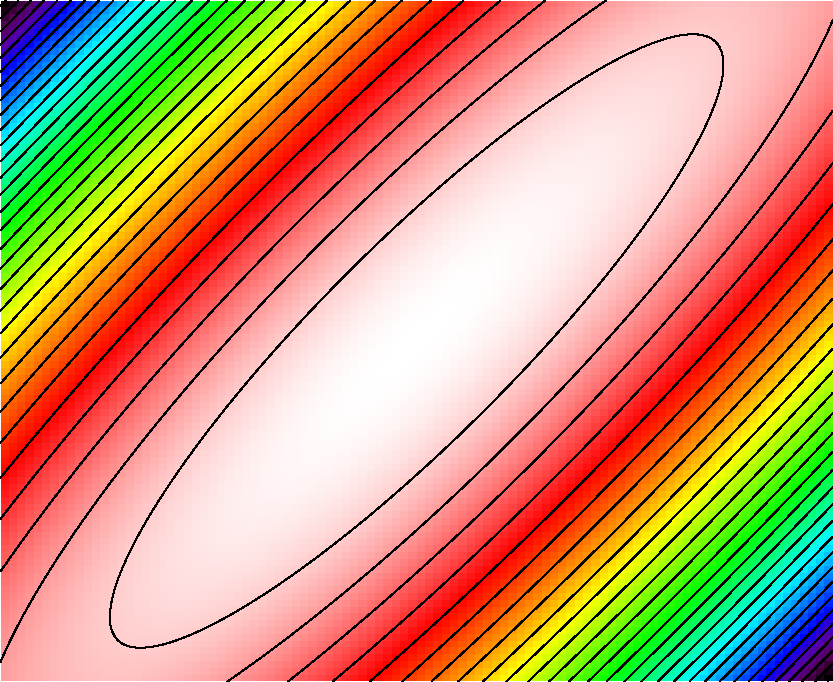
\includegraphics[width=\linewidth]{correlatedWeights}\pauseb\\
        Can't rescale coordinates\pauseb
      \end{center}
    \end{minipage}
\end{PauseHighLight}

\end{slide}


%%%%%%%%%%%%%%%%%%%%%%% Next Slide %%%%%%%%%%%%%%%%%%%%%%%

\begin{slide}
  \section{Correlated Weights}

  \begin{rightImage}{correlatedWeights}
    \begin{PauseHighLight}
      \begin{itemize}
      \item Correlated weights will lead to skewed valleys\pause
      \item Adaptive methods would be more efficient if they were
        rotationally invariant\pause
      \item However, this would slow down the algorithm\pause
      \item ADAM is a compromise between speed of implementation and
        effectiveness\pause
      \end{itemize}
    \end{PauseHighLight}

  \end{rightImage}

\end{slide}


%%%%%%%%%%%%%%%%%%%%%%% Next Slide %%%%%%%%%%%%%%%%%%%%%%%
\Outline %  Loss Landscape
%%%%%%%%%%%%%%%%%%%%%%% Next Slide %%%%%%%%%%%%%%%%%%%%%%%

\begin{slide}
\section[-2]{Loss Landscape}

\begin{PauseHighLight}
  \begin{itemize}\squeeze
  \item A useful concept for understanding optimisation is the loss
    landscape\pause
  \item For every value of the weights $\bm{w}$ there is some loss
    associated with it\pause
  \item Note that this landscape is very high dimensional, so our
    intuition can be a bit misleading\pause
  \item The landscape is also huge
  \end{itemize}
  \begin{center}
    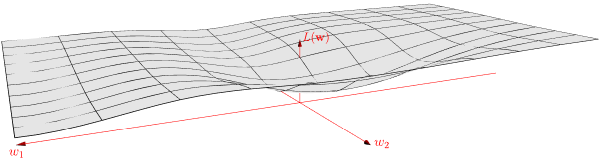
\includegraphics[width=0.9\linewidth]{lossLandscape.png}\pause
  \end{center}
\end{PauseHighLight}

\end{slide}

%%%%%%%%%%%%%%%%%%%%%%% Next Slide %%%%%%%%%%%%%%%%%%%%%%%

\begin{slide}
\section{Global and Local Minima}

\begin{PauseHighLight}
  \begin{itemize}
  \item Our objective is to minimise our loss\pause
  \item This would mean finding the global minimum\pause
  \item There are no algorithms that are guaranteed to find the global
    minimum\pause
  \item The best we can hope is to find a local minimum by doing
    gradient descent\pause
  \item In practice, our landscapes are so large that we are probably
    unable to find even a local minimum\pause
  \end{itemize}
\end{PauseHighLight}

\end{slide}

%%%%%%%%%%%%%%%%%%%%%%% Next Slide %%%%%%%%%%%%%%%%%%%%%%%

\begin{slide}
\section{Noisy Optimisation}

\begin{PauseHighLight}
  \begin{itemize}
  \item Because we are using mini-batches we aren't actually following
    the correct gradients\pause
  \item If we reduce our step size then our average gradient is closer
    to the true gradient\pause
  \item Thus our optimisation is inherently noisy\pause
  \item At least for deep learning there is no evidence that the
    weights stop changing even after learning for a huge amount of time\pause
  \end{itemize}
\end{PauseHighLight}

\end{slide}


%%%%%%%%%%%%%%%%%%%%%%% Next Slide %%%%%%%%%%%%%%%%%%%%%%%

\begin{slide}
\section{Valleys in Valleys in Valleys}

\begin{PauseHighLight}
  \begin{itemize}
  \item My view of the loss landscape is that we have valleys inside
    bigger valleys insider bigger valleys, and so on\pause
  \item If our noise is high (we use large step size), we can navigate
    away from local valleys and move towards the big valley\pause
  \item But, we can't explore the small valleys\pause
  \item Often when the rate of improvement slows down, practitioners
    will reduce their learning rate by a factor of 10 and the rate of
    improvement jumps up\pause
  \item Some practitioners cycle through raising and lowering their
    learning rates which may speed up convergence\pause
  \end{itemize}
\end{PauseHighLight}

\end{slide}

%%%%%%%%%%%%%%%%%%%%%%% Next Slide %%%%%%%%%%%%%%%%%%%%%%%

\begin{slide}
\section[-2]{Reducing the Step Size}
\pb
\pause
\pauselevel{=1}
\begin{center}
  \multipdf[width=0.7\linewidth]{valleyInValley}\pause
\end{center}
\begin{center}
  \multipdf[width=0.7\linewidth]{OUprocess}\pause
\end{center}

\end{slide}


%%%%%%%%%%%%%%%%%%%%%%% Next Slide %%%%%%%%%%%%%%%%%%%%%%%

\begin{slide}
\section[-2]{Symmetries}

\pb
\begin{itemize}
\item When training neural networks (deep or shallow) there are
  typically many symmetries\pauseh
\item Examples come from exchanging the weights of neurons (or
  filters in CNNs) in two layers\pauseh
  \begin{center}
    \multipdf[width=0.6\linewidth]{permutationSymmetry}\pause
  \end{center}
\end{itemize}

\end{slide}

%%%%%%%%%%%%%%%%%%%%%%% Next Slide %%%%%%%%%%%%%%%%%%%%%%%

\begin{slide}
\section[-2]{More Symmetries}

\begin{PauseHighLight}
  \begin{itemize}
  \item With $n$ hidden nodes there are $n!$ symmetries\pause
  \item Often if I multiply all the input and output weights to a node
    by $-1$ the network will be the same\pause
  \item There are also continuous symmetries.  For linear networks
    with two layers performing a mapping $\mat{W}_2 \mat{W}_1$ then
    for any invertible matrix $\mat{U}$ (where
    $\mat{U}\mat{U}^{-1}=\mat{I}$)
    \begin{align*}
      \mat{W}_2 \mat{W}_1 = \mat{W}_2  \,\mat{I} \, \mat{W}_1\pause
      = \mat{W}_2 \,(\mat{U}\,\mat{U}^{-1}) \mat{W}_1\pauseb
     = (\mat{W}_2 \,\mat{U})\,(\mat{U}^{-1} \mat{W}_1)\pauseb
    \end{align*}
    so a network with weights $\mat{W}_2'=\mat{W}_2 \,\mat{U}$ and
    $\mat{W}_1'=\mat{U}^{-1}\mat{W}_1$ will perform the same mapping\pause
  \item There will be a huge space of equivalent networks\pause
  \end{itemize}
\end{PauseHighLight}

\end{slide}

%%%%%%%%%%%%%%%%%%%%%%% Next Slide %%%%%%%%%%%%%%%%%%%%%%%

\begin{slide}
  \section[-2]{Skip Connections}

  \pb\pauselevel{=1 :30}\pause\pauselevel{=1}
  \begin{center}
    \multipdf[width=0.8\linewidth]{skipConnections}\pause
  \end{center}
  \begin{itemize}
  \item Breaks permutation symmetry\pause. Used in Resnets,
    transformer, etc.\pause
  \end{itemize}
\end{slide}



%%%%%%%%%%%%%%%%%%%%%%% Next Slide %%%%%%%%%%%%%%%%%%%%%%%

\begin{slide}
\section[-2]{Symmetries}

\pb\pause
\begin{minipage}{0.6\linewidth}
  \begin{itemize}
\item The landscape potentially has a huge manifold with the same
  losses (neutral network)\pauseh
\item Find solution close to start\pauseh \pauselevel{=30}
\item We should think of optimisation more as a process of
  travelling than a process of arriving\pauseh
\item Of course even if we do minimise our loss we are not
  guaranteed to minimise our generalisation performance\pauseh
\end{itemize}\hfill
\end{minipage}
\begin{minipage}{0.35\linewidth}\pauselevel{=3}
  \begin{flushright}
    \multipdf[width=0.85\linewidth]{symmetryLoss}\pause
  \end{flushright}
\end{minipage}

\end{slide}

%%%%%%%%%%%%%%%%%%%%%%% Next Slide %%%%%%%%%%%%%%%%%%%%%%%

\begin{slide}
\section{Lessons}

\begin{PauseHighLight}
  \begin{itemize}
  \item SGD together with automatic differentiation has revolutionised
    machine learning\pause
  \item There are a number of techniques to get the step size
    right\pause: momentum\pauseb, adaptive step size\pauseb,
    ADAM\pauseb
  \item Still need to understand that we are exploring a huge and
    complex loss landscape\pause
  \item What works is problem specific\pause{} (as always)\pauseb
  \end{itemize}
\end{PauseHighLight}

\end{slide}

%%% Local Variables:
%%% TeX-master: "lectures"
%%% End:
